%\textsl{}%!TEX TS-options = --shell-escape
%!TEX TS-program = pdflatex
\documentclass[%
   10pt,              % Schriftgroesse
   nenglish,           % wird an andere Pakete weitergereicht
   a4paper,           % Seitengroesse
   DIV11,             % Textbereichsgroesse (siehe Koma Skript Dokumentation !)
]{scrartcl}%     Klassen: scrartcl, scrreprt, scrbook, article
% -------------------------------------------------------------------------

\usepackage[utf8]{inputenc} % Font Encoding, benoetigt fuer Umlaute
\usepackage[english]{babel}   % \textsl{}Spracheinstellung

\usepackage[T1]{fontenc} % T1 Schrift Encoding
\usepackage{textcomp}    % Zusatzliche Symbole (Text Companion font extension)
\usepackage{lmodern,dsfont}     % Latin Modern Schrift
\usepackage{dsfont}
%\usepackage{wasysym}
\usepackage{ulem}
\usepackage{graphicx}
\usepackage{grffile} %allows to use pngs
\usepackage{eurosym}
%\usepackage{txfonts}
\usepackage{stmaryrd}
\usepackage{amsfonts}
\usepackage{amsmath}
\usepackage{hyperref}
\usepackage{tikz}
\usepackage{multirow}
\usepackage{listings}
\usepackage{etextools}
\usepackage{ifthen}
\usepackage{TikZ} %phylogenetischer Baum
\usetikzlibrary{calc, shapes, backgrounds} %für die Phylogenetische bäume
\usetikzlibrary{automata,arrows}
\usepackage{subfigure} 


% Definition des Headers
\usepackage{geometry}
\geometry{a4paper, top=3cm, left=3cm, right=3cm, bottom=3cm, headsep=0mm, footskip=0mm}
\renewcommand{\baselinestretch}{1.3}\normalsize

\def\header#1#2#3#4#5#6#7{\pagestyle{empty}
\noindent
\begin{minipage}[t]{0.6\textwidth}
\begin{flushleft}
\textbf{#4}\\% Fach
#6\\% Semester
Tutor: #2  % Tutor 
\end{flushleft}
\end{minipage}
\begin{minipage}[t]{0.4\textwidth}
\begin{flushright}
\points{#7}% Punktetabelle
\vspace*{0.2cm}
#5%  Names
\end{flushright}
\end{minipage}

\begin{center}
{\Large\textbf{ Blatt #1}} % Blatt

{(Abgabe am #3)} % Abgabedatum
\end{center}
}

\newenvironment{vartab}[1]
{
    \begin{tabular}{ |c@{} *{#1}{c|} } %\hline
}{
    \end{tabular}
}

\newcommand{\myformat}[1]{& #1}

\newcommand{\entry}[1]{
  \edef\result{\csvloop[\myformat]{#1}}
  \result \\ \hline
}

\newcommand{\numbers}[1]{
  \newcounter{ctra}
\setcounter{ctra}{1}
\whiledo {\value{ctra} < #1}%
{%
  \myformat{\thectra}
  \stepcounter{ctra}%
}
\myformat{\thectra}
}
\newcommand{\emptyLine}[1]{
  \newcounter{ctra1}
\setcounter{ctra}{1}
\whiledo {\value{ctra1} < #1}%
{%
  \myformat{\hspace*{0.5cm}}
  \stepcounter{ctra1}%
}
}

\newcommand{\points}[1]{
\newcounter{colmns}
\setcounter{colmns}{#1}
\stepcounter{colmns}
  \begin{vartab}{\thecolmns}
    \numbers{#1} & $\sum$\\\hline
    \emptyLine{\thecolmns}\\
  \end{vartab}
}


\begin{document}
%\header{Blatt}{Tutor}{Abgabedatum}{Vorlesung}{Bearbeiter}{Semester}{Anzahl Aufgaben}
\header{7}{Alexander Seitz}{26. October 2015}{Bioinformatics I}{\\Jonas Ditz \\\& Benjamin Schroeder}{WS 15/16}{3}

 \section*{Exercise 1 - \textsl{Hirschberg algorithm for alignment in linear space}}
  
  \begin{figure}[h]
  	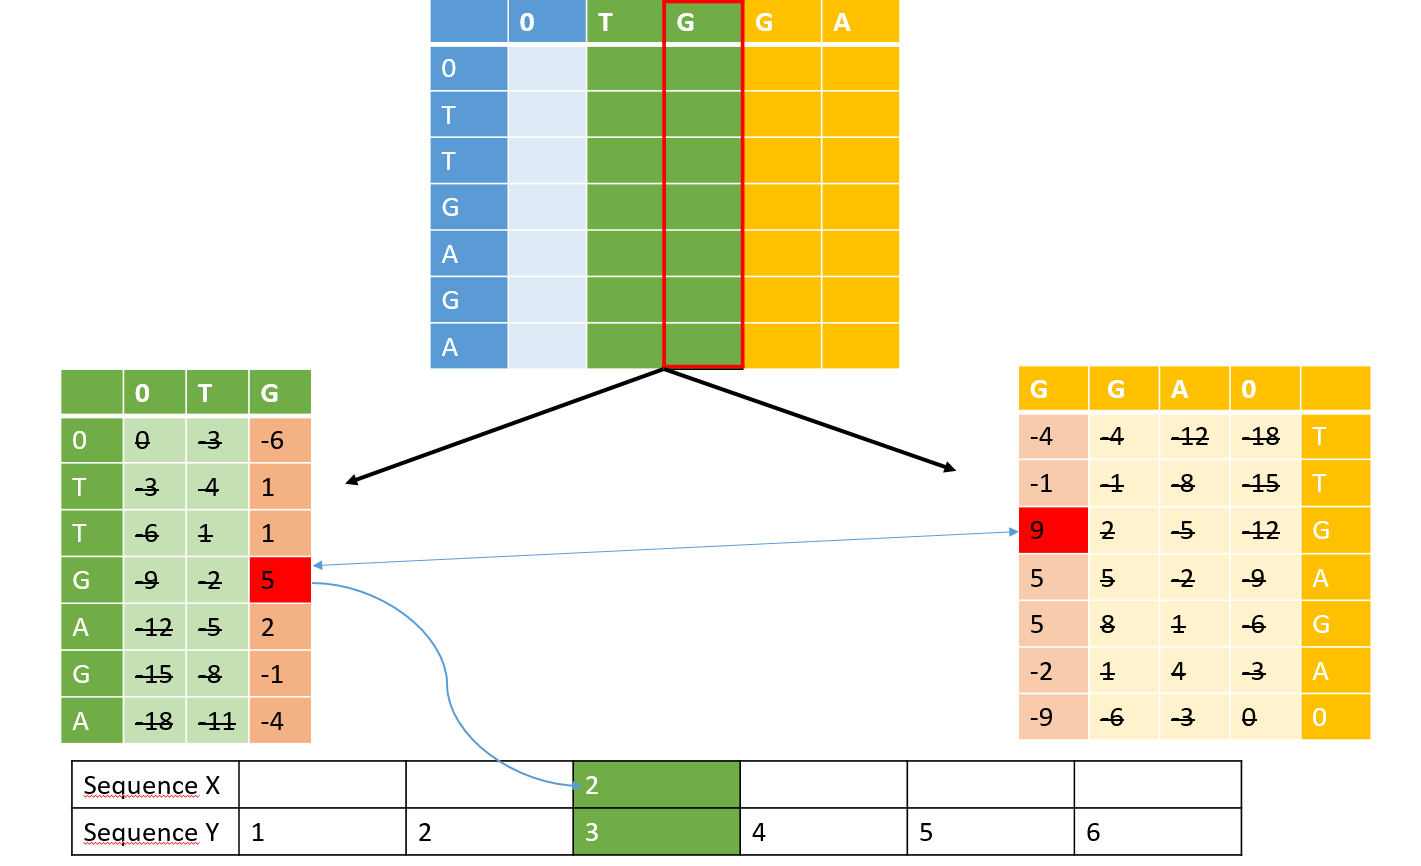
\includegraphics[scale=0.25]{img/Hirschberg_Step1.png}
  	\label{Step1}
  	\caption{BLAAAAAAAAAAA}
  \end{figure}
  
  \begin{figure}[h]
   	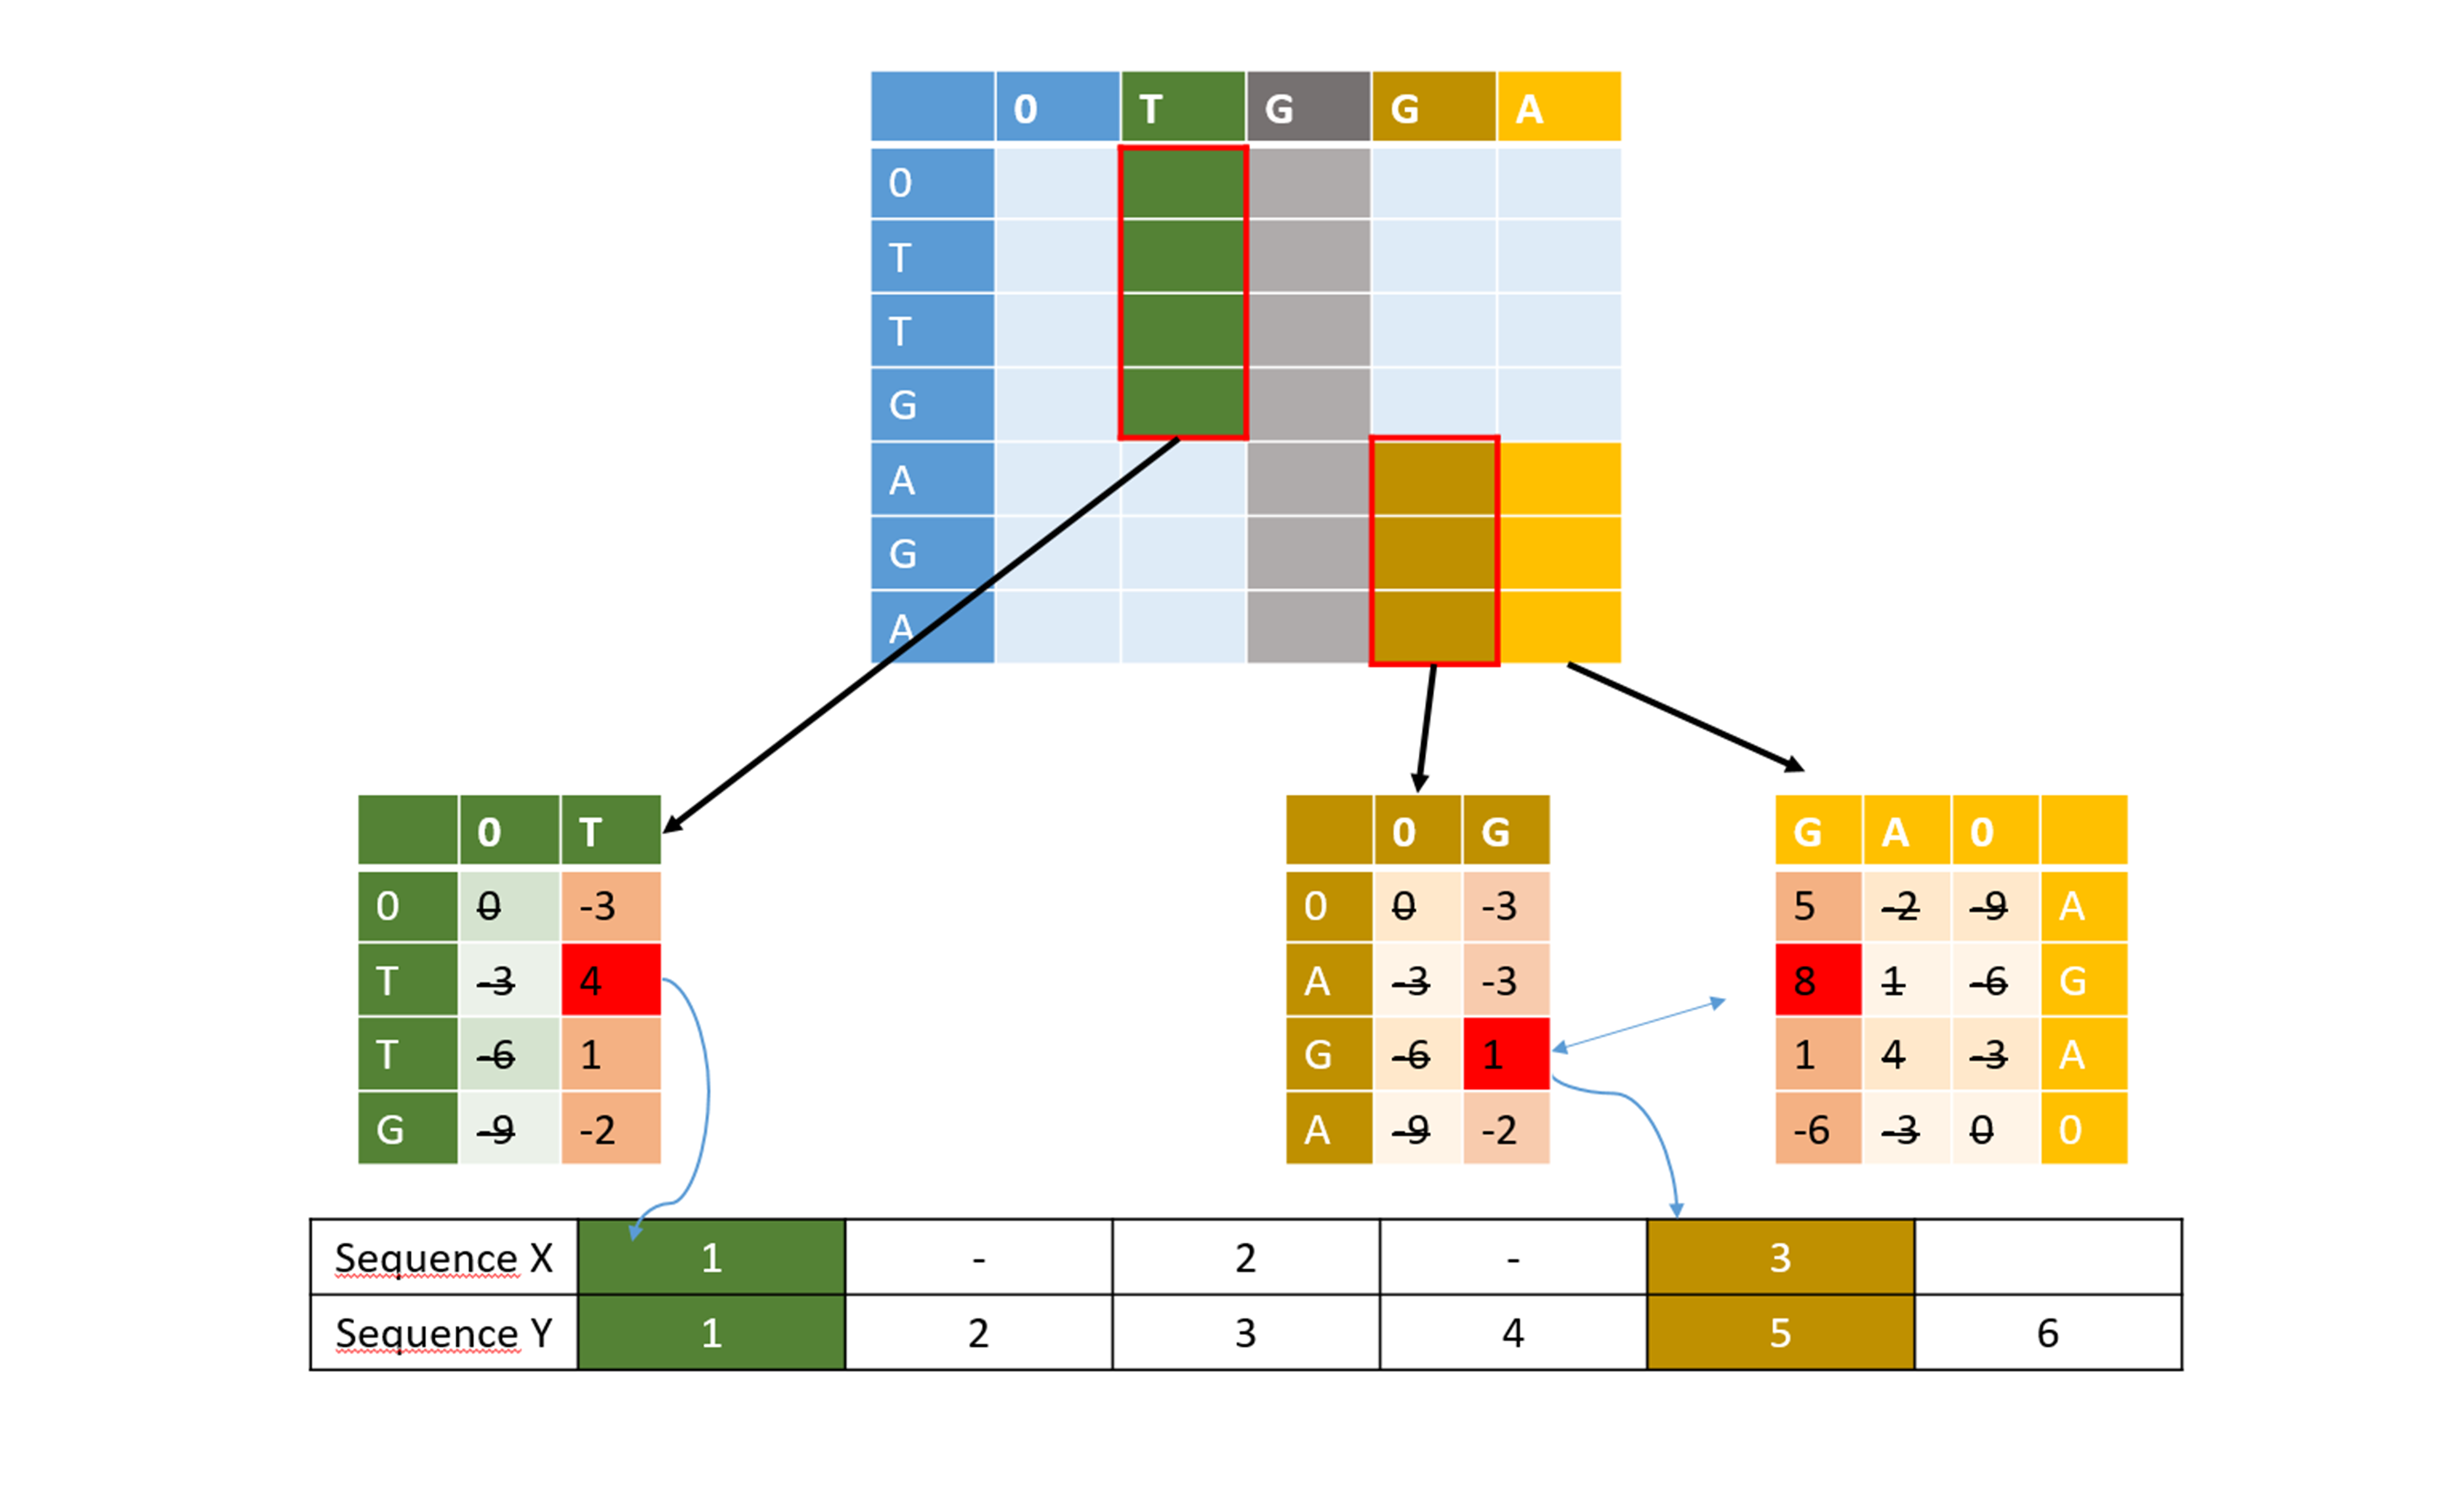
\includegraphics[scale=0.25]{img/Hirschberg_Step2.png}
   	\label{Step2}
   	\caption{BLAAAAAAAAAAA}
  \end{figure}
  \begin{figure}[h]
    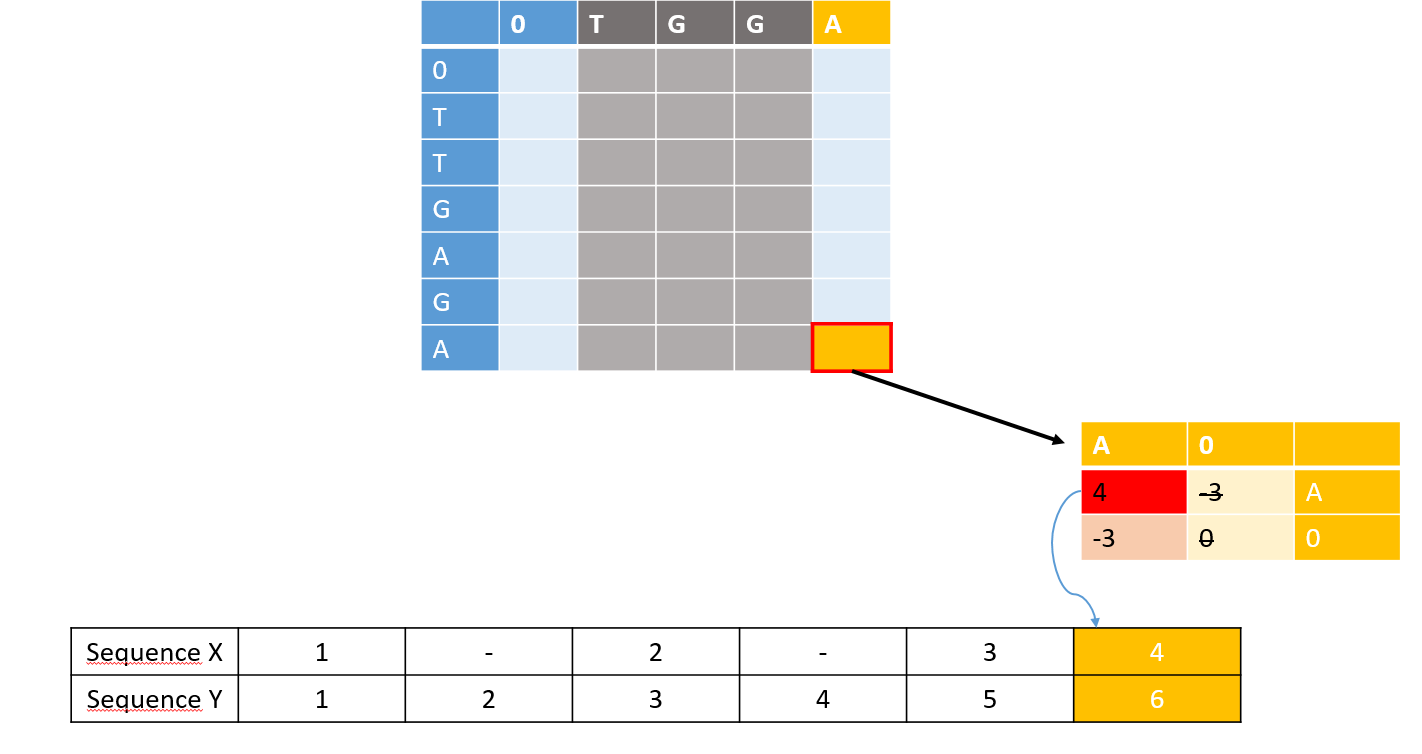
\includegraphics[scale=0.25]{img/Hirschberg_Step3.png}
	\label{Step3}
	\caption{BLAAAAAAAAAAA}
  \end{figure}
      
  \begin{figure}[h]
   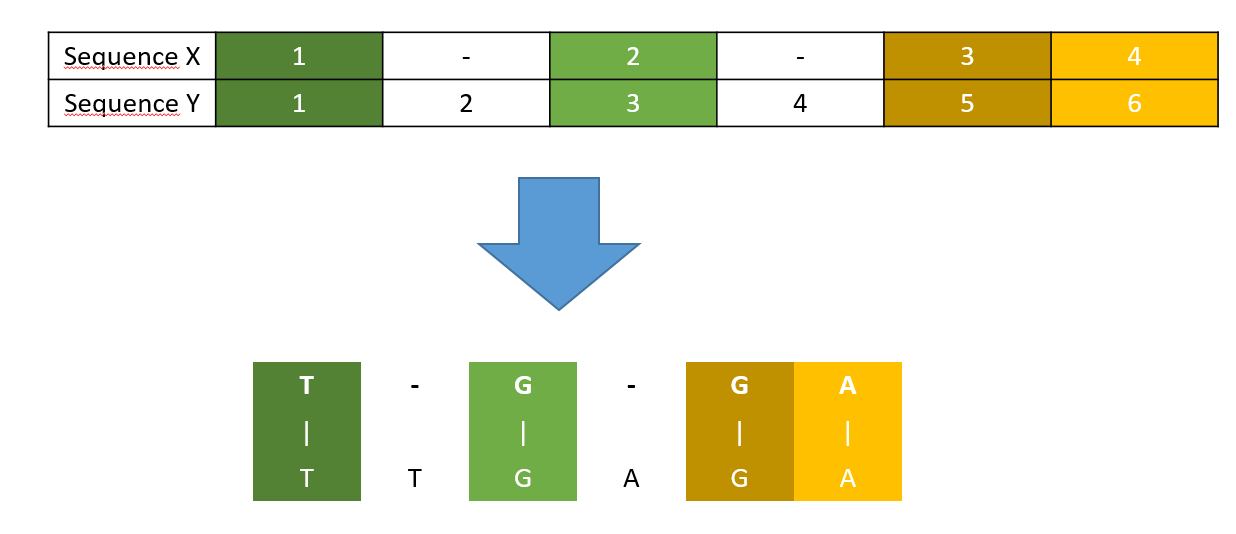
\includegraphics[scale=0.25]{img/Hirschberg_Step4.png}
   \label{Step4}
   \caption{BLAAAAAAAAAAA}
   \end{figure}
 \section*{Exercise 2 - \textsl{Do scoring matrices have expected score smaller than zero?}}
 
 The substitution matrices were evaluated according to the expectancy value formula given in the lecture, the substitution matrices were evaluated with the assumption of uniform distributed amino acids in two sequences.
 \begin{equation*}
 \sum_{a,b \in \Sigma}p_a p_b s(a,b)
 <=>  (\sum_{a,b \in \Sigma} s(a,b))  p_a p_b
 \label{expectance}
 \end{equation*}
 
 For the determination of one expectance value, $p_a$ and $p_b$ were each substituted with $1/20$, for the probabilistic occurrence in sequences with uniform distributed amino acids. The sum was calculated via R and the total summation of the substitution matrix \ref{expectance}.The result for each matrix can be seen in table \ref{Results-Expectance}.
 
 \begin{table}[h]
 \begin{tabular}{|c|c|}
 	\hline \rule[-2ex]{0pt}{5.5ex} Substitution Matrix & Expectance Value \\ 
 	\hline \rule[-2ex]{0pt}{5.5ex} BLSOUM50 & -1.155 \\ 
 	\hline \rule[-2ex]{0pt}{5.5ex} BLOSUM52 & -1.065 \\ 
 	\hline \rule[-2ex]{0pt}{5.5ex} BLOSUM80 & -2.3275 \\ 
 	\hline \rule[-2ex]{0pt}{5.5ex} PAM250 & -1.14 \\ 
 	\hline \rule[-2ex]{0pt}{5.5ex} PAMN & 0.155 \\ 
 	\hline 
 \end{tabular} 
 
   	\label{Results-Expectance}
   	\caption{Result of the calculation with each given substitution matrix according to equation}
 \end{table}
 
 As a conclusion we want to state, that all substitution matrices are possible feasible matrices. Except of the PAMN matrix, which has a positive expectancy value, which could lead to wrong conclusion.
One Aspect we also want to state, is that we did not calculate the values for the matrices with the unknown sign x or X. and the B or Z sign,  which stands for two amino acids. Although it would be possbile to use the unknown sign, if they are also uniform distributed in a sequence. But as a result of the wanted comparison, between matrices which didn't contain these signs, we did not use these columns and rows in our calculations.
 
 \section*{Exercise 3 - \textsl{Needleman-Wunsch algorithm for affine gap scores}}
 
  
\end{document}